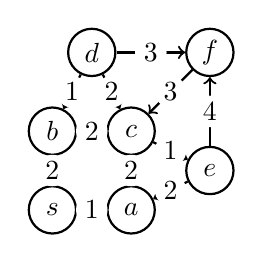
\begin{tikzpicture}[->, thick, main/.style = {circle,draw, inner sep = 0pt, minimum size = 0.6cm}, edge/.style = {circle, midway, fill=white, inner sep=0pt, minimum size=0.4cm}, scale = 0.5]    \node[main] (s) at (0, 0) {$s$};
    \node[main] (a) at (2, 0) {$a$};
    \node[main] (b) at (0, 2) {$b$};
    \node[main] (c) at (2, 2) {$c$};
    \node[main] (d) at (1, 4) {$d$};
    \node[main] (e) at (4, 1) {$e$};
    \node[main] (f) at (4, 4) {$f$};
    \path
        (d) edge[bend right = 0] node[edge] {3} (f)
        (f) edge[bend right = 0] node[edge] {3} (c)
        (d) edge[bend right = 0] node[edge] {1} (b)
        (b) edge[bend right = 0] node[edge] {2} (c)
        (c) edge[bend right = 0] node[edge] {2} (a)
        (s) edge[bend right = 0] node[edge] {2} (b)
        (s) edge[bend right = 0] node[edge] {1} (a)
        (d) edge[bend right = 0] node[edge] {2} (c)
        (e) edge[bend right = 0] node[edge] {4} (f)
        (c) edge[bend right = 0] node[edge] {1} (e)
        (e) edge[bend right = 0] node[edge] {2} (a);
\end{tikzpicture}